\chapter{Testando as Malhas de Controle}
\label{chap:testesMalhas}
Para alcançar o objetivo final deste trabalho, fez-se uma modularização do problema que foi validada e integrada, módulo a módulo. Primeiramente será testada a malha 1 de controle de velocidade angular das rodas. Ou seja, após dado um comando de velocidade angular para roda quanto tempo a malha levará para estabilizar o sistema convergindo-o para zero. 

O primeiro teste a ser realizado será na malha de controle mais interna com cinco controladores diferentes: P, PI, PID, Incremental e o quinto, através de uma função polinomial que converte a velocidade angular desejada na potência a ser aplicada. Para utilizar essa função polinomial é necessário recorrer a um método da linguagem \emph{NXC} de ativação dos motores que já implementa um controlador de malha fechada. Essa função foi obtida através de um mapeamento das potências aplicadas e as velocidades adquiridas pelo motor, daí então foi realizada uma aproximação de 4º grau. %Esse mapeamento, assim como, a função aproximada foi realizada pelo Professor Tales Argolo Jesus e será utilizada neste trabalho.

Para que a malha de controle interno cumpra com seu objetivo é necessário que o erro entre a velocidade desejada e a velocidade real em cada roda tenda a zero. Ou seja, desejando-se que o robô tenha uma velocidade linear de $0.1 m/s$ e uma velocidade angular de $0.6 rad/s$, faz-se uma conversão desses valores utilizando da \autoref{eq:convVelAngRodas}, encontrando os valores desejados para cada uma das rodas. Feito isso, calcula-se o erro entre a velocidade desejada e a real de cada roda e passa esse erro como entrada para o controlador que deve aplicar uma potência nos motores pretendendo atingir a velocidade desejada.

Para realizar o teste com a malha interna foram aplicadas três entradas distintas e foi observado o tempo de conversão do sistema para um estado estacionário e se o sistema estava convergindo para um erro próximo de zero. Utilizando-se de um tempo amostral de cerca de 25 milissegundos, aplicou nas primeiras 100 amostras uma velocidade linear e angular nula, feito isso nas próximas 400 amostras aplicou-se uma velocidade linear de $0.189 m/s$ e uma velocidade angular nula (velocidade angular de cada roda igual a $8.75 rad/s$) e nas 500 amostras seguintes manteve-se a velocidade linear anterior e foi acrescentado uma velocidade angular de $0.628 rad/s$ (sendo, $10.38 rad/s e 7.12 rad/s$, as velocidades angulares das rodas direita e esquerda, respectivamente). Sendo que no primeiro momento o robô deve permanecer parado, adquirir uma velocidade linear e caminhar em linha reta com uma velocidade de $0.189 m/s$, para então iniciar uma trajetória circular de raio de $30 cm$ e período de $10 s$.

\section{Malha 1: Controlador Incremental}
\label{m1ContInc}

Primeiro a malha interna foi testada com um controlador incremental que consiste basicamente em aumentar ou diminuir a potência das rodas, conforme o erro. Se o erro for positivo, acrescenta o incremento, se for negativo faz-se a potência menos o incremento. Foram testados os seguintes valores como incremento: 1, 3 e 6 e como podemos observar nos gráficos \ref{fig:contInc1},\ref{fig:contInc6} e \ref{fig:contInc3} e na \autoref{t:cinc}, o controlador de incremento igual a um é suave e possui oscilações aceitáveis mas, o tempo para estabilização do sistema é maior que o dobro do tempo obtido com o incremento igual a seis. Entretanto, o controlador com incremento igual a seis é muito agressivo, oscilando o dobro de vezes se comparado ao controlador de incremento igual a um. 

Fazendo-se o incremento igual a 3 tem-se um custo-benefício interessante pois, o sistema continua razoavelmente suave, com oscilações bem próximas ao do controlador de incremento igual a um e com um tempo de resposta o dobro de vezes mais rápido. Já, comparado ao de incremento igual a seis, ele possui um tempo de resposta bem próximo e com a metade da oscilação, com um controle bem mais suave. Sendo, o mais adequado para a malha interna se comparado ao controlador com outros valores de incremento. 

\begin{table}[!htb]
	\centering
	\begin{tabular}{|c|c|c|c|}
		\hline
		\begin{tabular}[c]{@{}c@{}}Características/\\ Incrementos\end{tabular} & \textbf{\begin{tabular}[c]{@{}c@{}}Oscilação\\ ($rad/s$)\end{tabular}} & \textbf{\begin{tabular}[c]{@{}c@{}}Tempo de \\ Ajuste ($s$)\end{tabular}} & \textbf{Controle} \\ \hline
		\textbf{1}                                                             & $\pm 0.6 rad/s$                                                            & $\approx 2s$                                                                      & Suave             \\ \hline
		\textbf{3}                                                             & $\pm 0.6 rad/s$                                                            & $\approx 1s$                                                                      & Suave             \\ \hline
		\textbf{6}                                                             & $\pm 1.2 rad/s$                                                            & $\approx 0.75s$                                                                   & Agressivo         \\ \hline
	\end{tabular}
	\caption{Malha1: Controlador Incremental}
	\label{t:cinc}
\end{table}

\begin{figure}[!htb]
	\centering
	\begin{subfigure}{.5\textwidth}
		\centering
		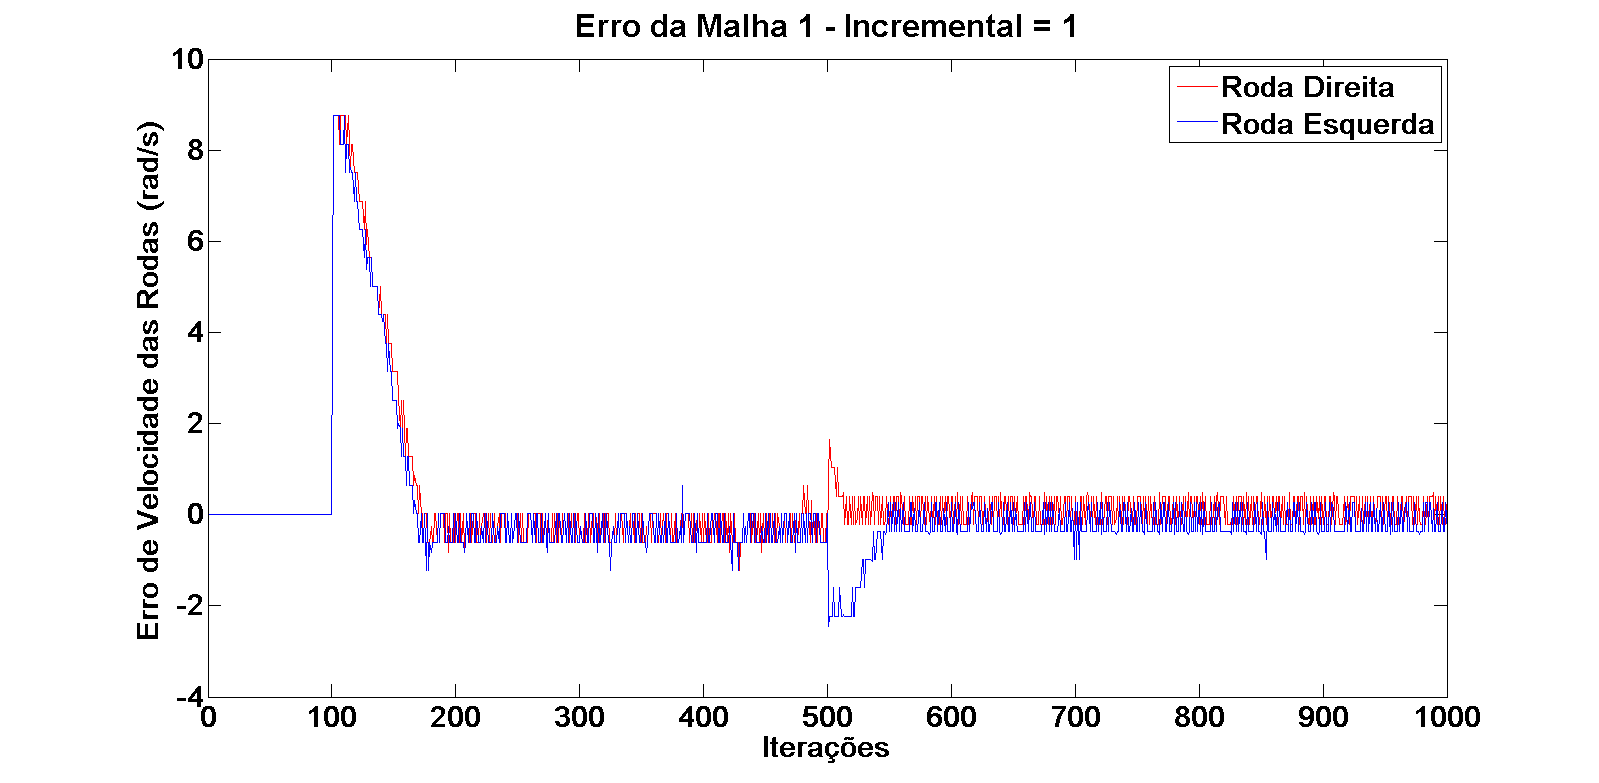
\includegraphics[width=.9\linewidth]{./Testes/Malha1/Incremental/Malha1_Inc1}
		\caption{Incremento = 1}
		\label{fig:contInc1}
	\end{subfigure}%
	\begin{subfigure}{.5\textwidth}
		\centering
		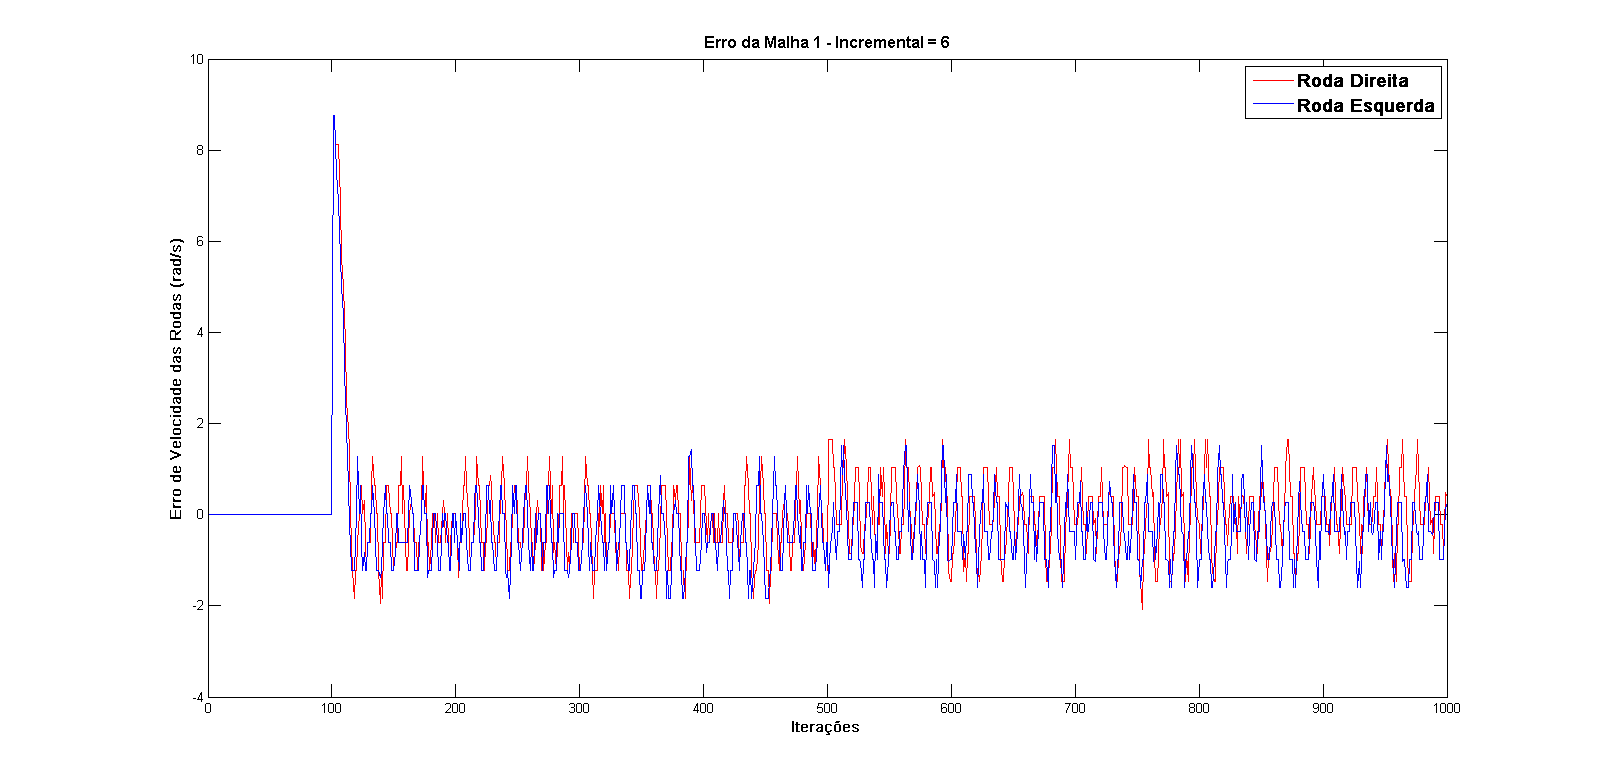
\includegraphics[width=.9\linewidth]{./Testes/Malha1/Incremental/Malha1_Inc6}
		\caption{Incremento = 6}
		\label{fig:contInc6}
	\end{subfigure}
	\begin{subfigure}{1.0\textwidth}
		\centering
		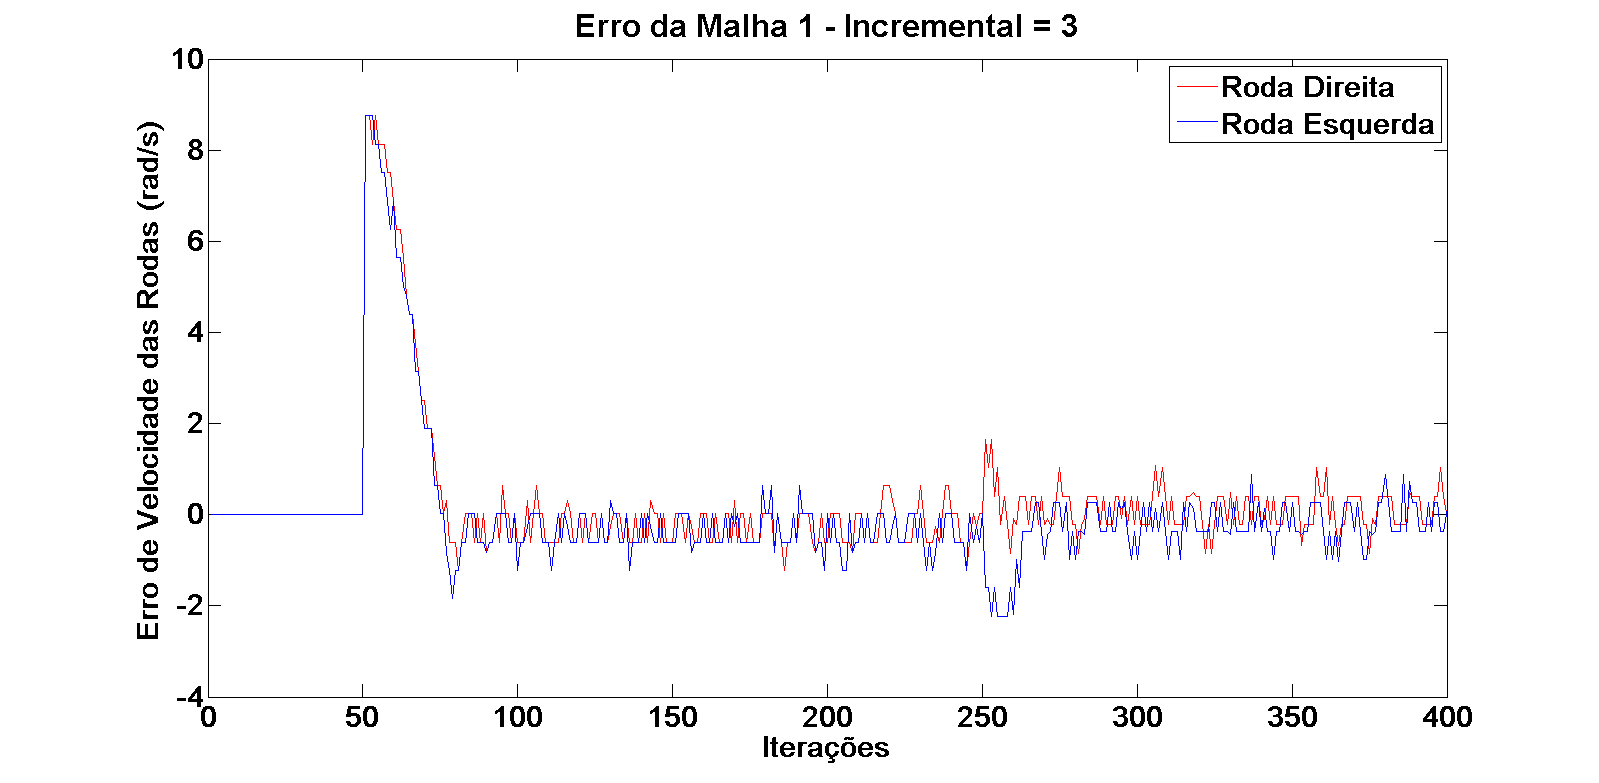
\includegraphics[width=.9\linewidth]{./Testes/Malha1/Incremental/Malha1_Inc3}
		\caption{Incremento = 3}
		\label{fig:contInc3}
	\end{subfigure}
	\caption{Experimentos com Controlador Incremental}
	\label{fig:contInc}
\end{figure}

\section{Malha 1: Controladores P, PI e PID}
\label{m1ContPID}

Foram realizados testes com controladores do tipo P, PI e PID, os ganhos foram ajustados de forma empírica e a \autoref{t:cpid}, assim como a \autoref{fig:contPID} mostram alguns dos resultados  obtidos. Pode-se observar que o melhor ganho obtido a partir dos testes realizados foi o do controlador PID com ganho proporcional igual a 10, ganho integrativo igual a 15 e ganho derivativo igual a 0.2, visto que ele apresentou o menor tempo de resposta com uma oscilação razoável. 

\begin{table}[!htb]
	\centering
	\begin{tabular}{|c|c|c|c|c|}
		\hline
		\textbf{\begin{tabular}[c]{@{}c@{}}Características/\\ Ganhos do controlador\end{tabular}} & \textbf{\begin{tabular}[c]{@{}c@{}}Estabiliza\\ ($rad/s$)\end{tabular}} & \textbf{\begin{tabular}[c]{@{}c@{}}Oscilação\\ ($rad/s$)\end{tabular}} & \textbf{\begin{tabular}[c]{@{}c@{}}Tempo de \\ Ajuste ($s$)\end{tabular}} & \textbf{Controle} \\ \hline
		\textbf{P: 10}                                                                            & $3$ $rad/s$                                                               & $1.3 rad/s$                                                            & $0.5s$                                                                    & Suave             \\ \hline
		\textbf{P:10 - I:15}                                                                      & $0$ $rad/s$                                                               & $0.65 rad/s$                                                           & $2s$                                                                      & Suave             \\ \hline
		\textbf{P:10 - I:17}                                                                      & $0$ rad/s                                                               & $0.6 rad/s$                                                            & $1.9s$                                                                    & Suave             \\ \hline
		\textbf{P:10 - I:15 - D:0.2}                                                              & $0$ $rad/s$                                                               & $1.3 rad/s$                                                            & $1.5s$                                                                    & Suave             \\ \hline
		\textbf{P:10 - I:15 - D:0.6}                                                              & $0$ $rad/s$                                                               & $0.65 rad/s$                                                           & $2s$                                                                      & Agressivo         \\ \hline
	\end{tabular}
	\caption{Experimentos com Controlador P/PI/PID}
	\label{t:cpid}
\end{table}


\begin{figure}[!htb]
	\centering
	\begin{subfigure}{.5\textwidth}
		\centering
		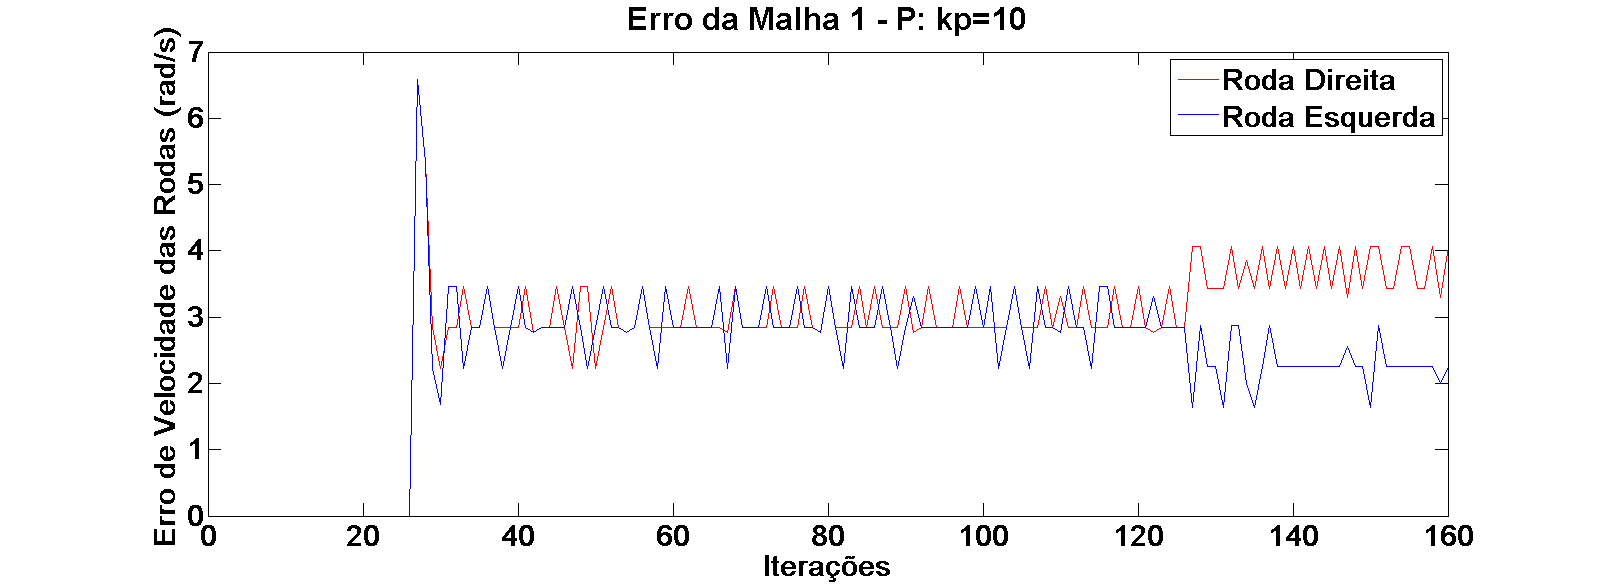
\includegraphics[width=.9\linewidth]{./Testes/Malha1/PID/m1_kp10}
		\caption{Controlador Proporcional (kp = 10)}
		\label{fig:contP}
	\end{subfigure}%
	\begin{subfigure}{.5\textwidth}
		\centering
		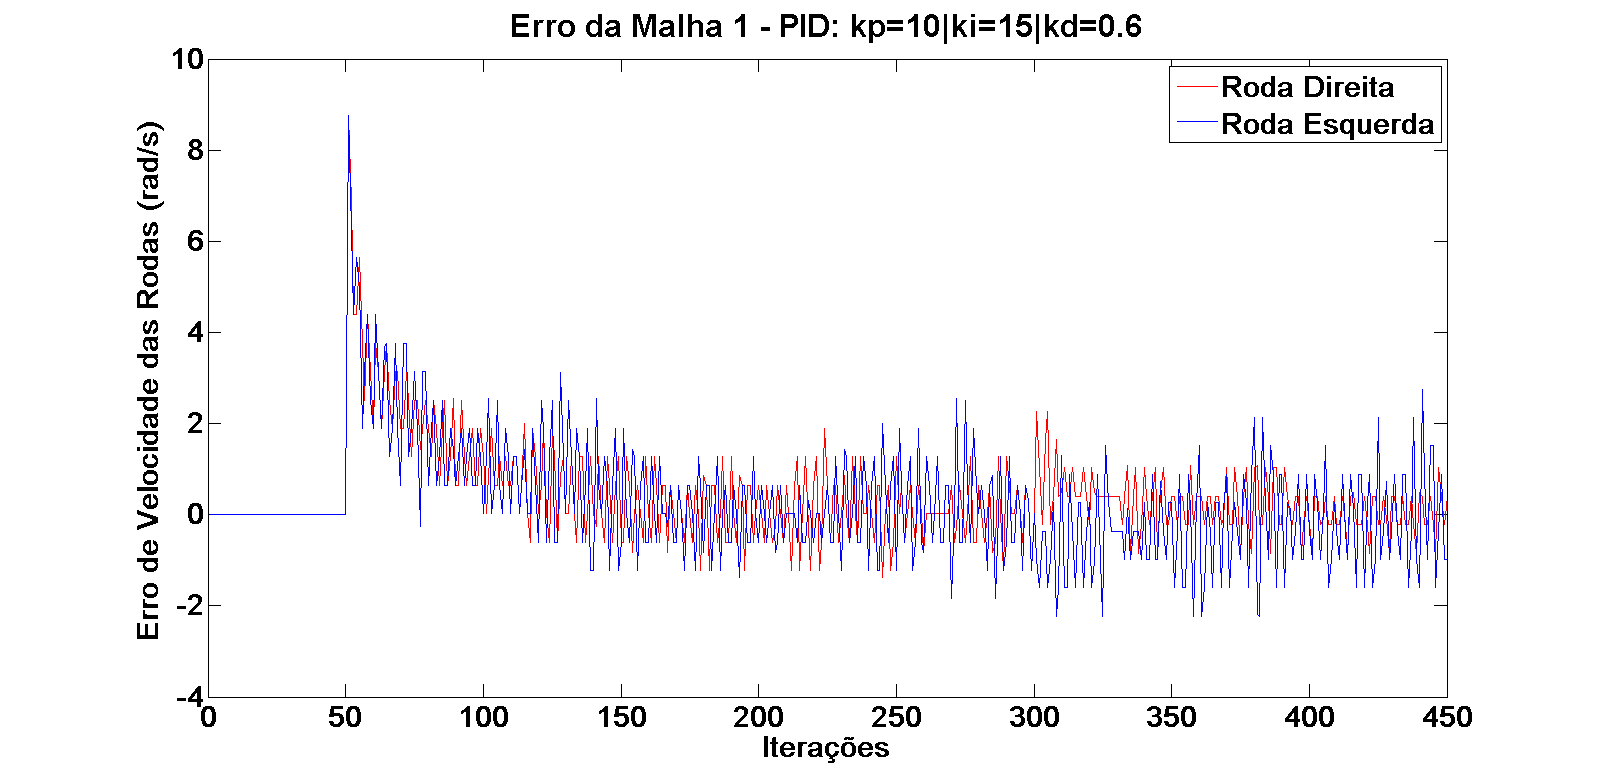
\includegraphics[width=.9\linewidth]{./Testes/Malha1/PID/m1_kp10ki15kd06}
		\caption{Controlador Proporcional - Integral - Derivativo (kp = 10, ki = 15 e kd = 0.6)}
		\label{fig:contPID2}
	\end{subfigure}
	\begin{subfigure}{0.5\textwidth}
	\centering
	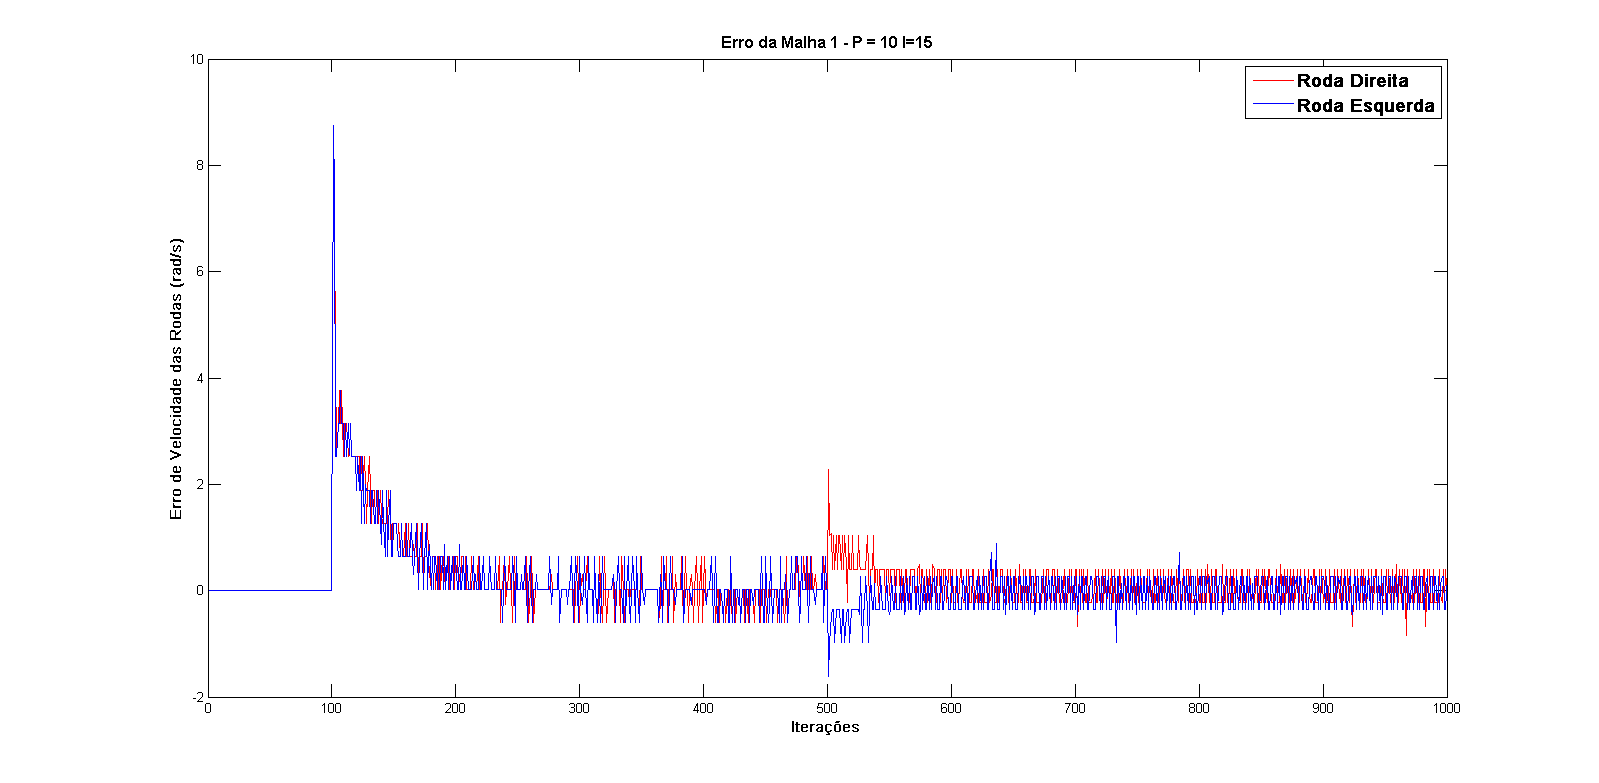
\includegraphics[width=.9\linewidth]{./Testes/Malha1/PID/m1_kp10ki15}
	\caption{Controlador Proporcional - Integral (kp = 10 e ki = 15)}
	\label{fig:contPI1}
	\end{subfigure}%
	\begin{subfigure}{0.5\textwidth}
	\centering
	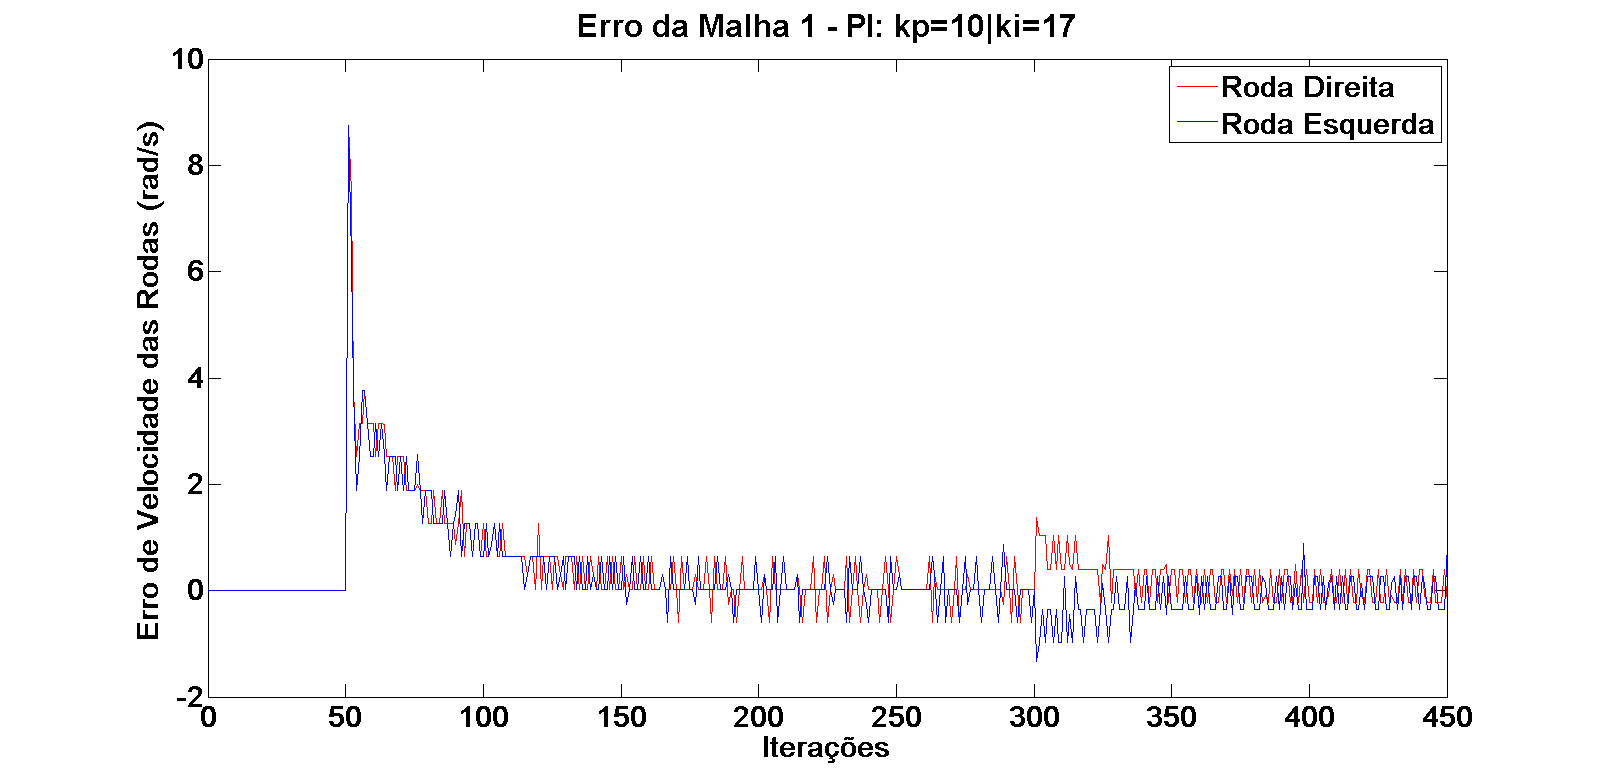
\includegraphics[width=.9\linewidth]{./Testes/Malha1/PID/m1_kp10ki17}
	\caption{Controlador Proporcional - Integral - Derivativo (kp = 10 e ki = 17)}
	\label{fig:contPI2}
	\end{subfigure}
	\begin{subfigure}{1.0\textwidth}
		\centering
		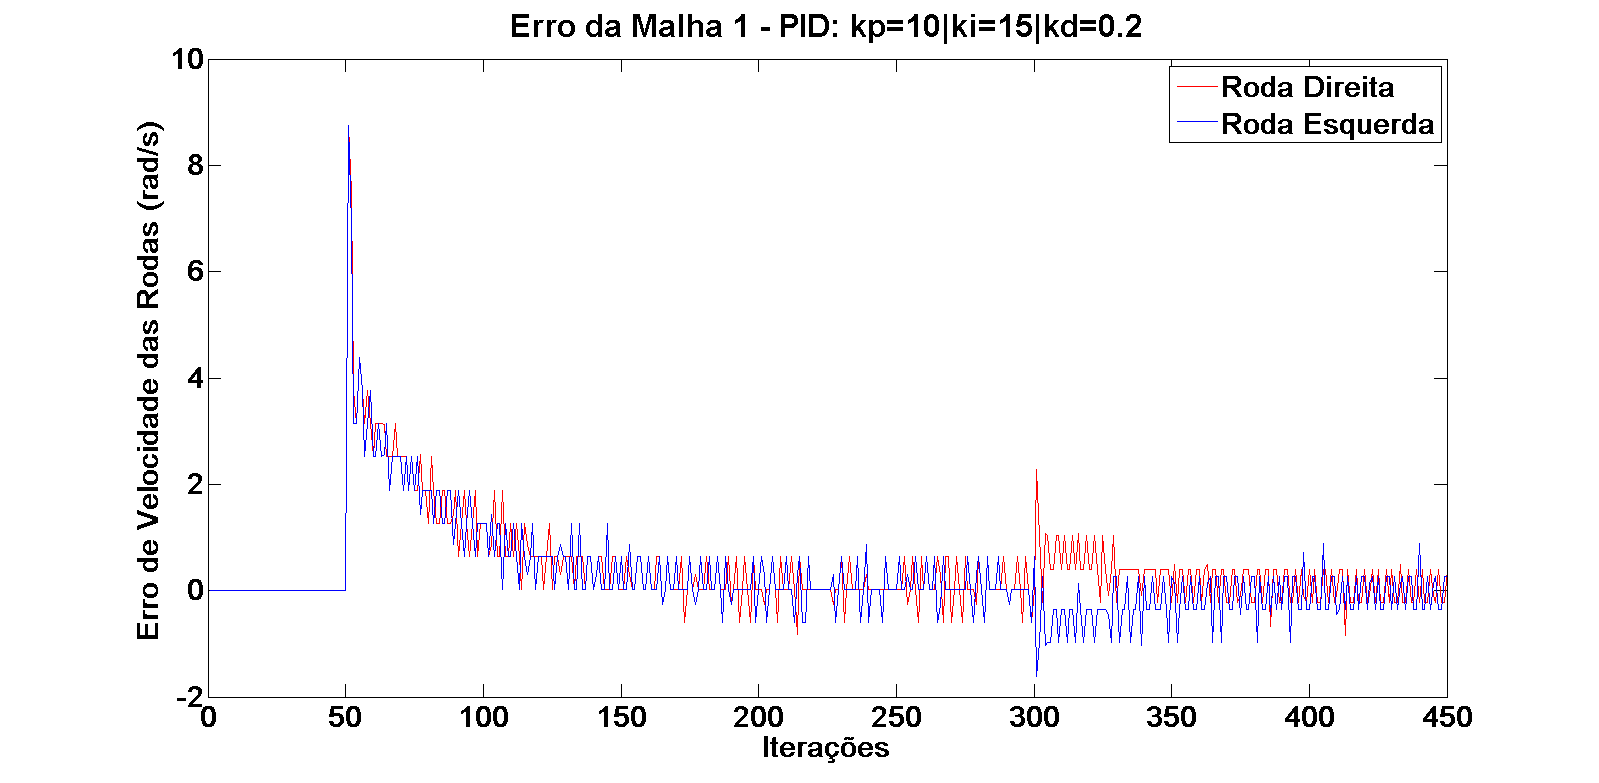
\includegraphics[width=.9\linewidth]{./Testes/Malha1/PID/m1_kp10ki15kd02}
		\caption{Controlador Proporcional - Integral - Derivativo (kp = 10, ki = 15 e kd = 0.2)}
		\label{fig:contPIDP}
	\end{subfigure}
	\caption{Experimentos com Controlador P/PI e PID}
	\label{fig:contPID}
\end{figure}

\section{Malha 1: Função de Ajuste Polinomial e Controlador Embutido}
\label{m1ContPol}
%Como já dito anteriormente, esse método utiliza de uma função polinomial que é um mapeamento aproximado da resposta dos motores aos diversos parâmetros de potência, tal como a \autoref{eq:pol}. Essa função foi obtida %pelo professor Tales Argolo 
%aplicando diversas potências ao motor e verificando a velocidade que o mesmo adquiria com esses comandos, feito isso foi utilizado o \emph{MATLAB\textregistered} para achar uma função aproximada de 4º grau. É importante constatar aqui que esse método utiliza um método da própria plataforma que implementa internamente um controlador, onde independente do peso contido no motor, ele adquiri a mesma velocidade para determinada potência(Função: \emph{OnFwdReg}).
Como já dito anteriormente, a plataforma já implementa uma malha de controle da velocidade dos motores, um controlador \emph{PID} já ajustado pelo fabricante, para utilizá-la basta usar um método específico da linguagem \emph{NXC}. Entretanto, a referência desta malha de controle é uma variável que assume valores entre -100 e 100, surge daí a necessidade de se fazer um mapeamento entre esta variável e a variável de velocidade angular assumida pelo motor em radianos por segundo. Para realizar este mapeamento estático, utiliza-se o método dos quadrados mínimos para se ajustar um polinômio de quarto grau aos dados medidos, obtendo a função mostrada na \autoref{eq:pol}.

\begin{equation}
f(\omega_{desejada}) = -0.00091\omega_{desejada}^{4} + 0.0223\omega_{desejada}^{3} - 0.01537\omega_{desejada}^{2} + 6.1864\omega_{desejada} - 0.0546
\label{eq:pol}
\end{equation} 
 
 Como pode ser visto na \autoref{fig:pol}, a função mapeia muito bem as saídas do motor, o sistema converge para um estado de erro nulo com um tempo de aproximadamente 2 segundos, com uma oscilação de $\pm0.6 rad/s$, bem próximo aos resultados obtidos com o controlador PI ajustado manualmente.
 
 \begin{figure}[!htb]
 	\centering
	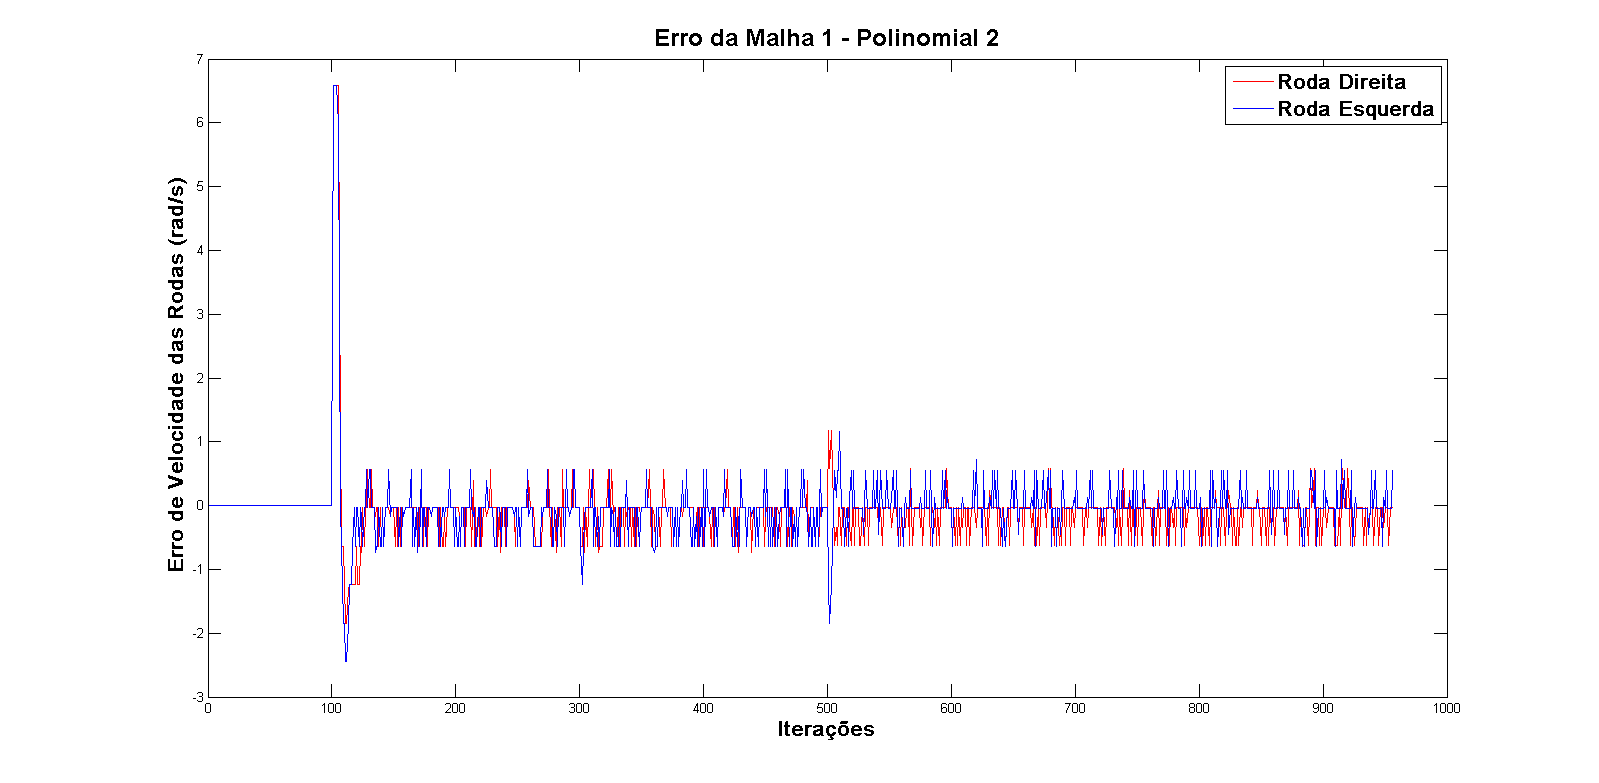
\includegraphics[width=.9\linewidth]{./Testes/Malha1/Polinomial/Polinomial}
 	\caption{Experimentos com a Função Polinomial e o Controlador PID Embutido}
 	\label{fig:pol}
 \end{figure}
 
 \section{Malha 2: Controle de Posicionamento}
 \label{m2}
 Nesta parte do trabalho, será mostrado os testes realizados com a segunda malha de controle, ela é responsável pela posição do robô. Ou seja, a malha recebe como referência a posição onde deseja-se que o robô esteja, a partir daí calcula-se a velocidade angular necessária para que o robô chegue ao ponto desejado. E esta então é passada para malha de controle interno. 
 
 Os testes foram realizados da seguinte maneira: O robô foi iniciado no ponto ($0.8,0.0$) e foi definido um alvo na origem do sistema que esse robô teria que circundar com um raio de 30 centímetros e um período de 24 segundos. Após mil e duzentas amostras, o raio e o período do sistema mudam sendo 40 centímetros de raio em um período de 30 segundos, tornando o teste muito parecido com o segundo problema em sí.
 
 Na \autoref{t:compMalha2} mostram alguns dos resultados obtidos pelos experimentos feitos com a segunda malha, utilizando-se o controlador proporcional de ganho unitário e com ganho proporcional igual a 2 na malha intermediária. Como já sabido, quando tem-se um controle em cascata é necessário que a malha interna responda pelo menos 5 vezes mais rápido do que a malha externa, quanto mais rápido melhor.
 
 Tendo isto em mente, %pode-se dizer que o a segunda malha de controle utilizando como controlador da malha interna o controlador polinomial, possui uma malha interna cerca de 7 vezes mais rápida do que a malha externa. Já com os controladores Incremental e PID são cerca de 14 e 11 vezes mais rápida, respectivamente.
 %Dessa forma, 
 do ponto de vista de tempo de resposta, todas atendem com o pré-requisito, no entanto, ao observar o sistema na vida real é possível notar que o controlador PID é muito agressivo e por vezes dá um tranco no motor, o que não é desejado, visto que qualquer comando brusco pode ocasionar em derrapagem das rodas, o que poderia levar o robô a se perder e mapear uma trajetória diferente da trajetória apresentada no mundo real.
 
 Os dois que apresentaram melhores resultados foram o controlador da malha externa proporcional com ganho de $\pm2$ combinados com os controladores Incermental e Polinomial. O que se confirma pelas figuras \ref{} e pela \autoref{t:CompMalha2}. Como mostrado na \autoref{}, os testes com controlador PI na malha intermediária não apresentaram um bom resultado, apresentando oscilações indesejadas que demoraram para se estabilizar ao mudar a ação de controle drasticamente, além de apresentar um controle mais agressivo.
 
 \begin{table}[!htb]
 	\centering
 	\begin{tabular}{|l|l|l|l|}
 		\hline
 		\textbf{\begin{tabular}[c]{@{}l@{}}Características/\\ Controlador Interno e Externo\end{tabular}}          & \textbf{\begin{tabular}[c]{@{}l@{}}Estabiliza em\\ ($rad$)\end{tabular}} & \textbf{\begin{tabular}[c]{@{}l@{}}Termpo de \\ Ajuste ($s$)\end{tabular}} & \textbf{Controle}                                          \\ \hline
 		\textbf{\begin{tabular}[c]{@{}l@{}}Incremental (Incremento 3)/\\ Proporcional (kp = 1.0)\end{tabular}}     & $\pm 0.3rad$                                                                & $\pm 14 s$                                                                     & Suave                                                      \\ \hline
 		\textbf{\begin{tabular}[c]{@{}l@{}}PID (kp = 10;ki = 15;kd = 0.2)/\\ Proporcional (kp = 1.0)\end{tabular}} & $\pm0.3 rad$                                                                 & $\pm17.5 s$                                                                   & Agressivo                                                  \\ \hline
 		\textbf{\begin{tabular}[c]{@{}l@{}}Polinomial/\\ Proporcional (kp = 1.0)\end{tabular}}                     & $\pm 0.3rad$                                                                    & $\pm 17.5 s$                                                                   & Suave                                                      \\ \hline
 		\textbf{\begin{tabular}[c]{@{}l@{}}Incremental (Incremento 3)/\\ Proporcional (kp = 2.0)\end{tabular}}     & $\pm 0.18 rad$                                                                   & $\pm 11 s$                                                                     & \begin{tabular}[c]{@{}l@{}}Pouco \\ Agressivo\end{tabular} \\ \hline
 		\textbf{\begin{tabular}[c]{@{}l@{}}Polinomial/\\ Proporcional (kp = 2.0)\end{tabular}}                     & $\pm 0.17 rad$                                                                   & $\pm 14 s$                                                                     & Suave                                                      \\ \hline
 	\end{tabular}
 	\caption{Comparativo dos Controladores da Malha Intermediária}
 	\label{t:compMalha2}
 \end{table}
 
 \begin{figure}[!htb]
 	\centering
 	\begin{subfigure}{1.0\textwidth}
 		\centering
 		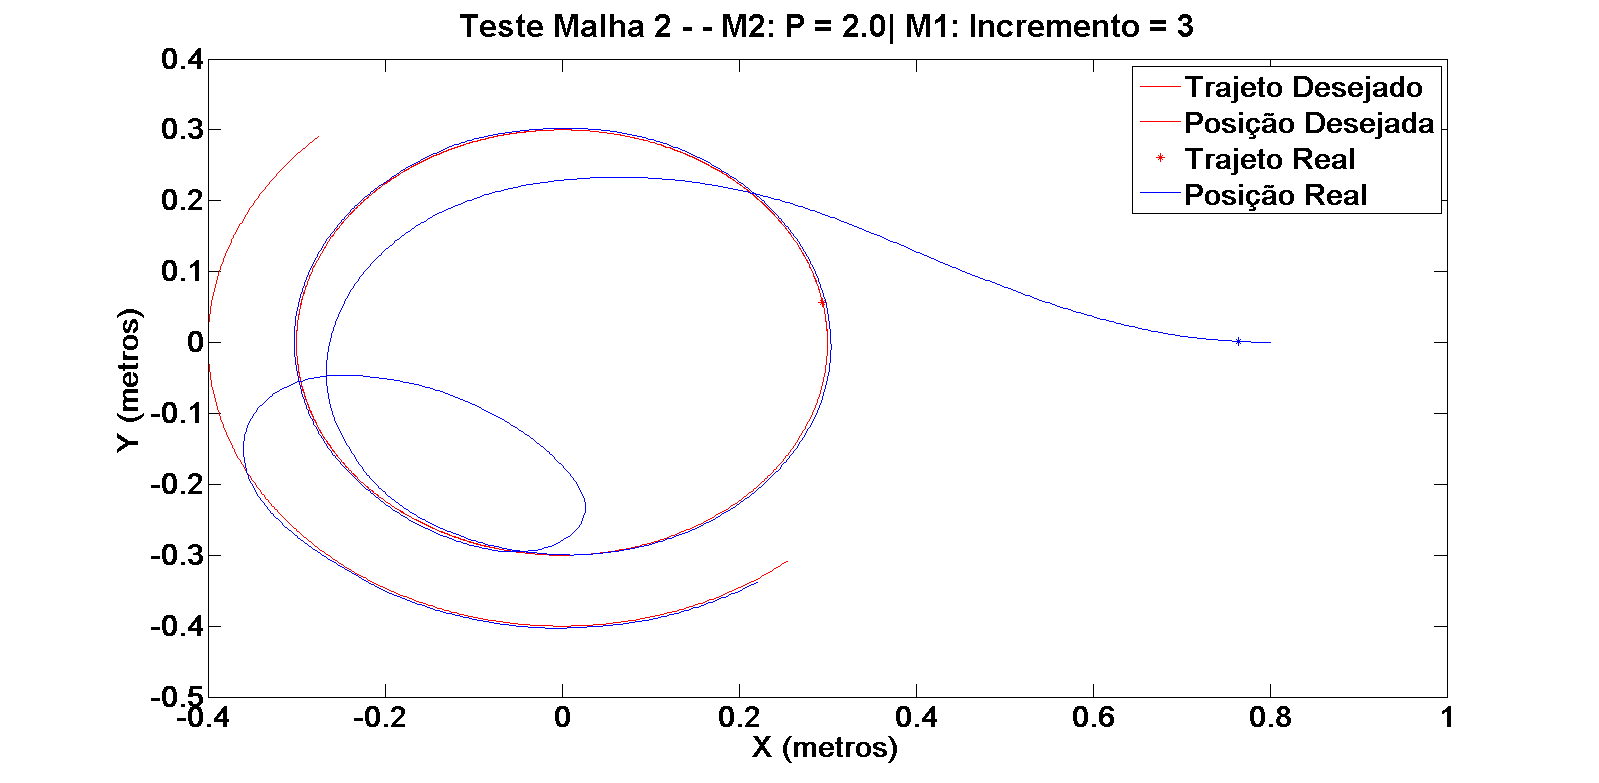
\includegraphics[width=.9\linewidth]{./Testes/Malha2/P2.0/Incremental-3/m2PosInc}
 		\caption{Malha Intermediária: P=2.0 - Malha Interna: Incremental k = 3}
 		\label{fig:m2incpos}
 	\end{subfigure}
 	\begin{subfigure}{1.0\textwidth}
 		\centering
 		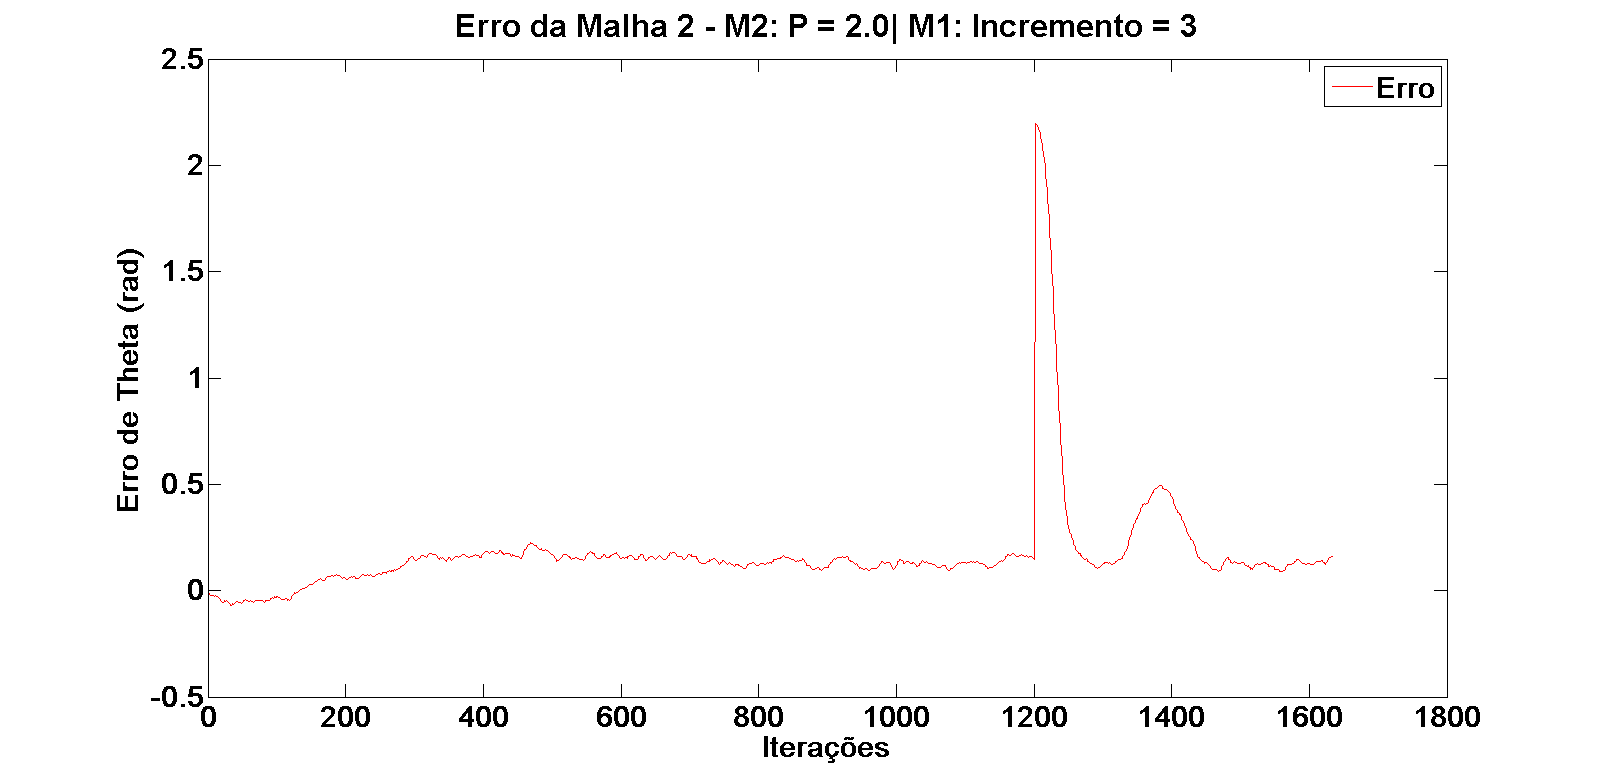
\includegraphics[width=.9\linewidth]{./Testes/Malha2/P2.0/Incremental-3/ErroM2Inc}
 		\caption{Erro da Malha Intermediária: P=1.0 - Malha Interna: Incremental k = 3}
 		\label{fig:m2incerr}
 	\end{subfigure}
 	\caption{Experimentos com a Malha Intermediária com Controlador Proporcional(kp=2.0) e Malha Interna: Controlador Incremental}
 	\label{fig:m2inc}
 \end{figure}
 
  \begin{figure}[!htb]
  	\centering
  	\begin{subfigure}{1.0\textwidth}
  		\centering
  		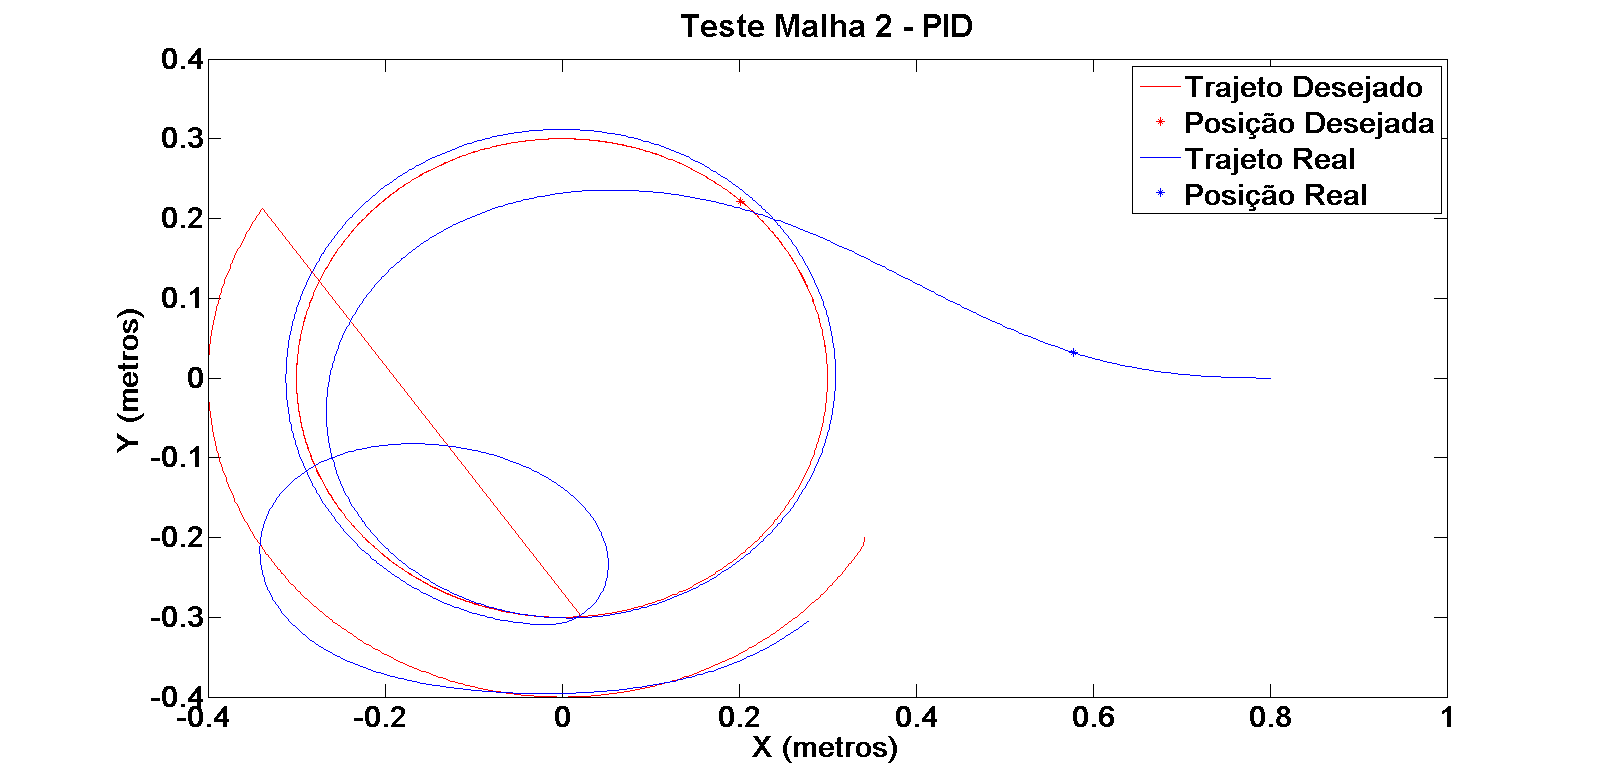
\includegraphics[width=.9\linewidth]{./Testes/Malha2/P1.0/PID/PIDPos}
  		\caption{Malha Intermediária: P=1.0 - Malha Interna: PID (kp = 10;ki = 15; kd = 0.2)}
  		\label{fig:m2pidpos}
  	\end{subfigure}
  	\begin{subfigure}{1.0\textwidth}
  		\centering
  		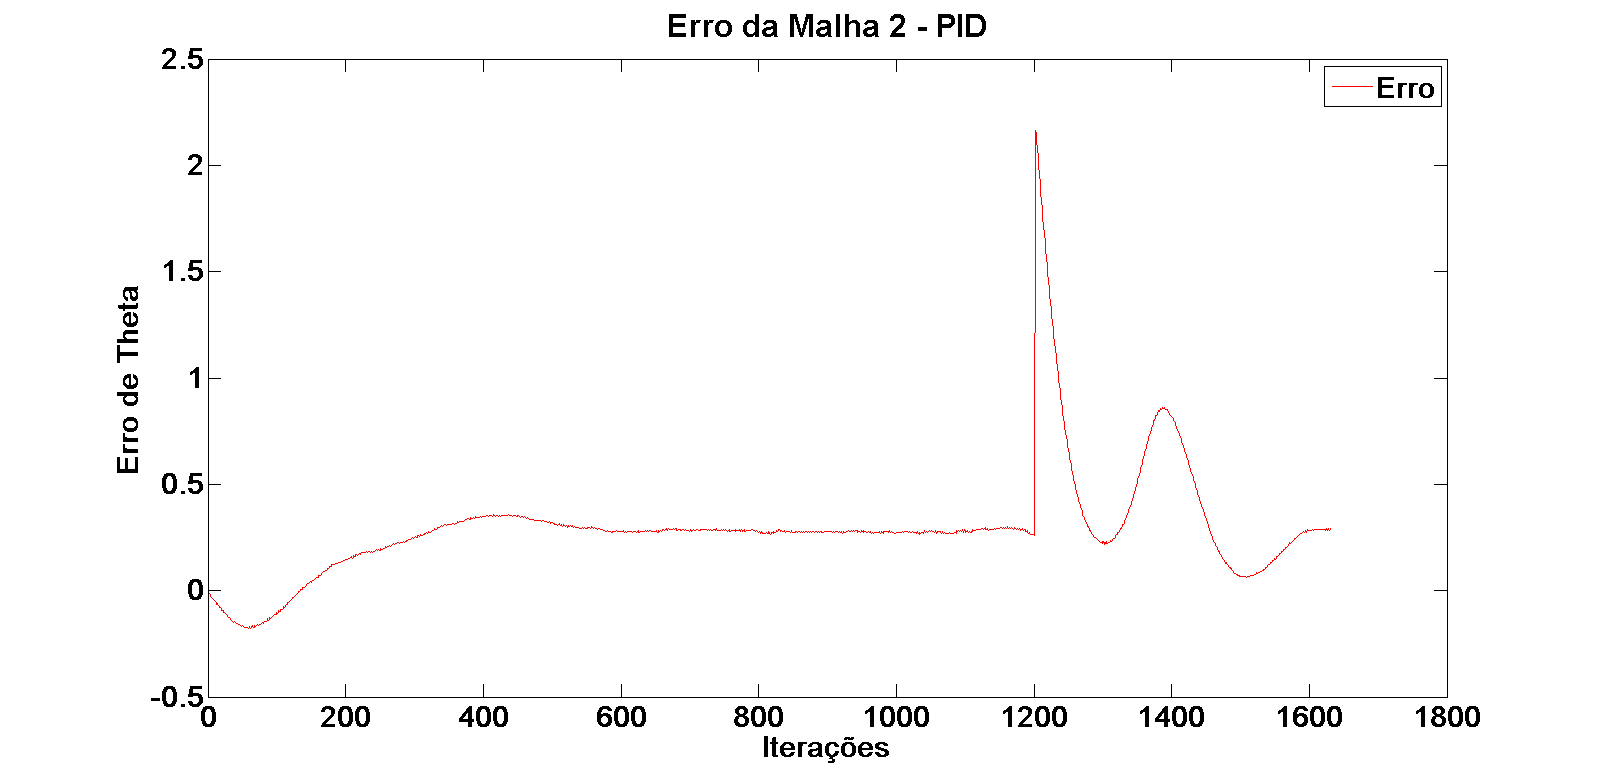
\includegraphics[width=.9\linewidth]{./Testes/Malha2/P1.0/PID/ErroThetaPID}
  		\caption{Erro da Malha Intermediária: P=1.0 - Malha Interna: PID (kp = 10;ki = 15; kd = 0.2)}
  		\label{fig:m2piderr}
  	\end{subfigure}
  	\caption{Experimentos com a Malha Intermediária com Controlador Proporcional e Malha Interna: Controlador PID}
  	\label{fig:m2pid}
  \end{figure}
  
    \begin{figure}[!htb]
    	\centering
    	\begin{subfigure}{1.0\textwidth}
    		\centering
    		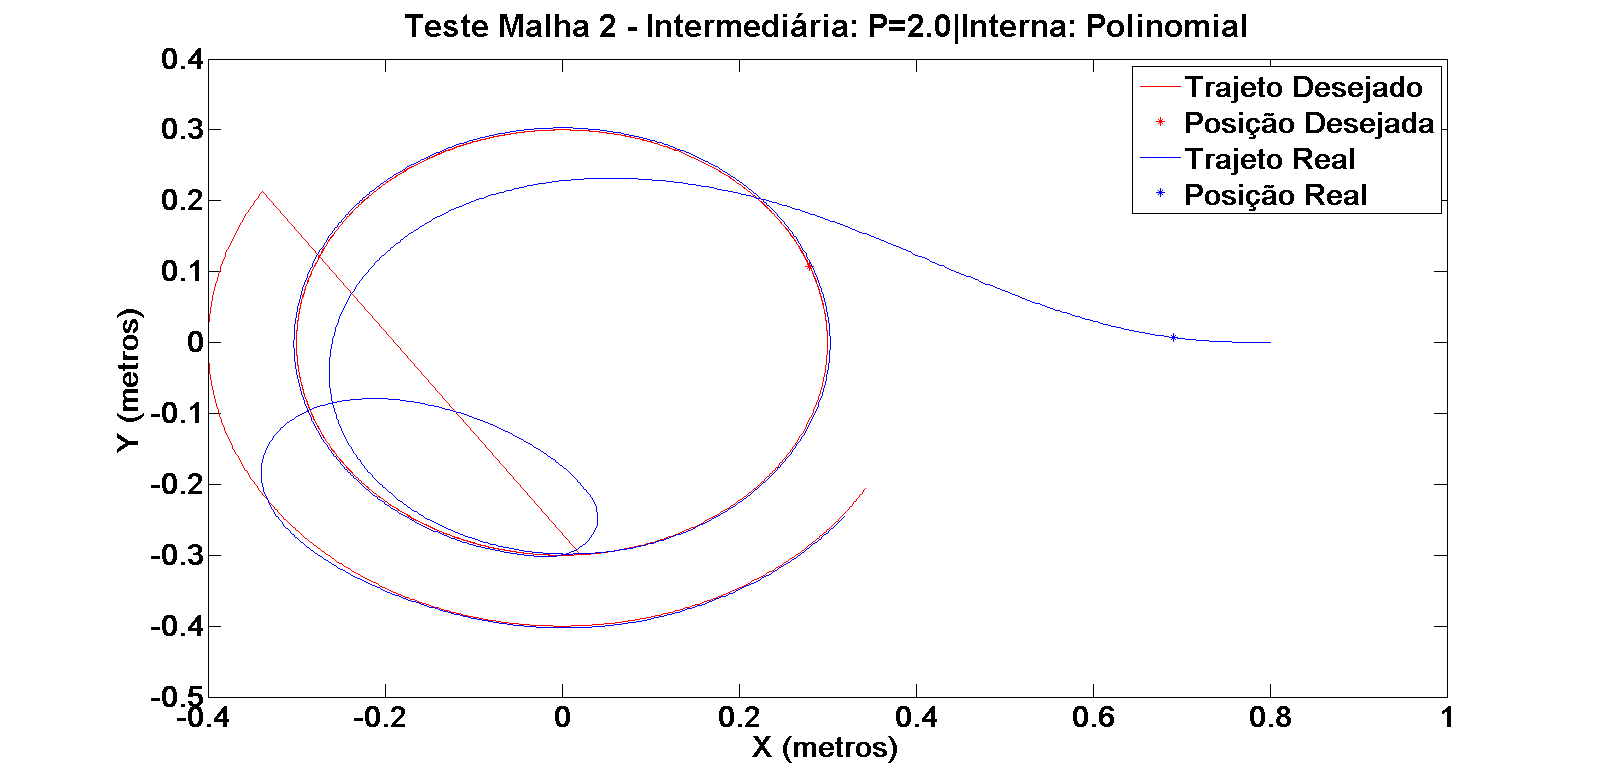
\includegraphics[width=.9\linewidth]{./Testes/Malha2/P2.0/Polinomial/m2PosPol}
    		\caption{Malha Intermediária: P=2.0 - Malha Interna: Polinomial}
    		\label{fig:m2polpos}
    	\end{subfigure}
    	\begin{subfigure}{1.0\textwidth}
    		\centering
    		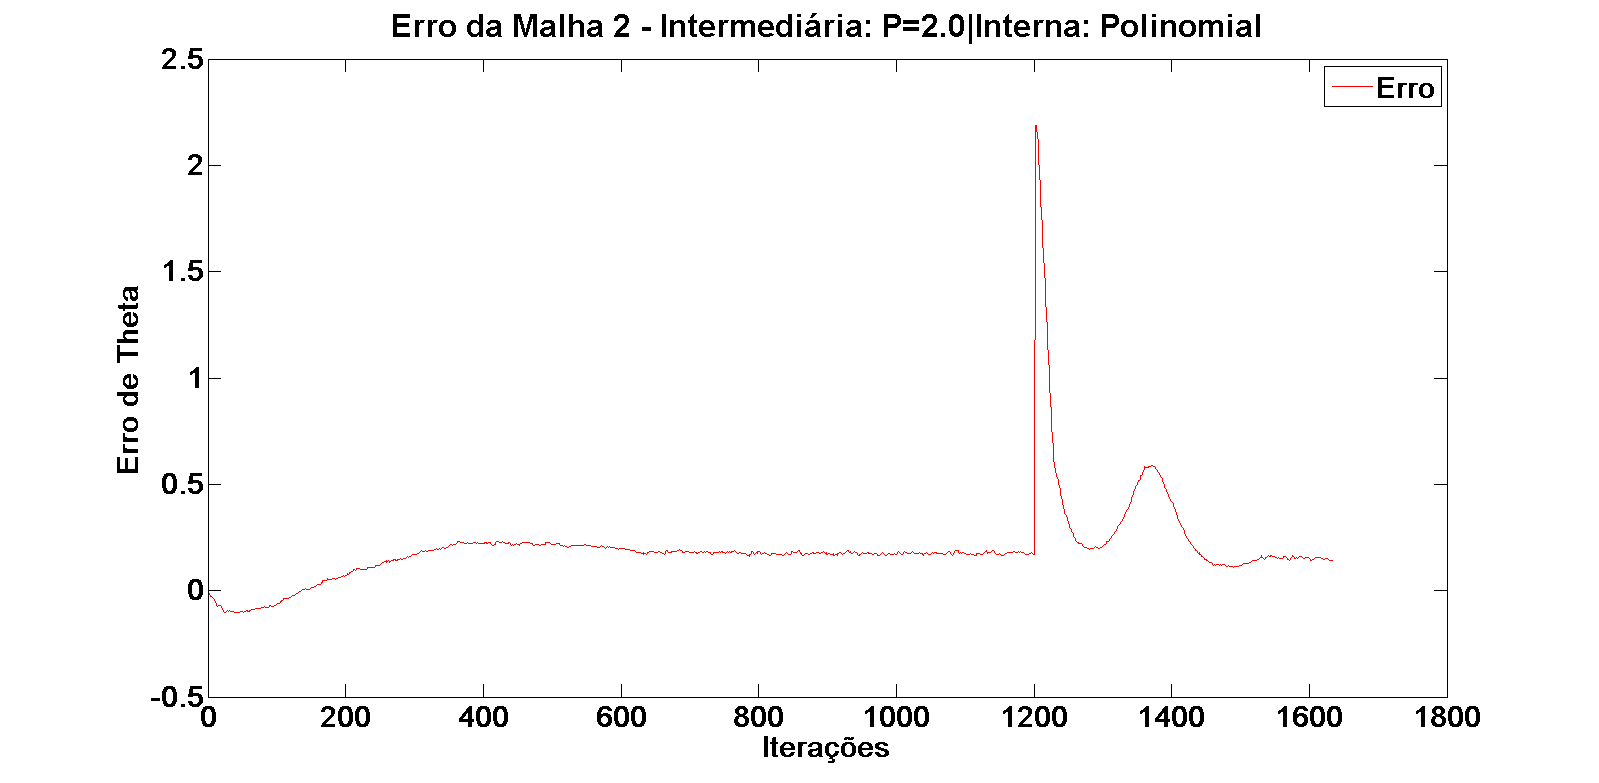
\includegraphics[width=.9\linewidth]{./Testes/Malha2/P2.0/Polinomial/m2ErroTheta}
    		\caption{Erro da Malha Intermediária: P=2.0 - Malha Interna: Polinomial}
    		\label{fig:m2piderr}
    	\end{subfigure}
    	\caption{Experimentos com a Malha Intermediária com Controlador Proporcional e Malha Interna: Controlador Polinomial}
    	\label{fig:m2pol}
    \end{figure}
 
    \begin{figure}[!htb]
    	\centering
    	\begin{subfigure}{1.0\textwidth}
    		\centering
    		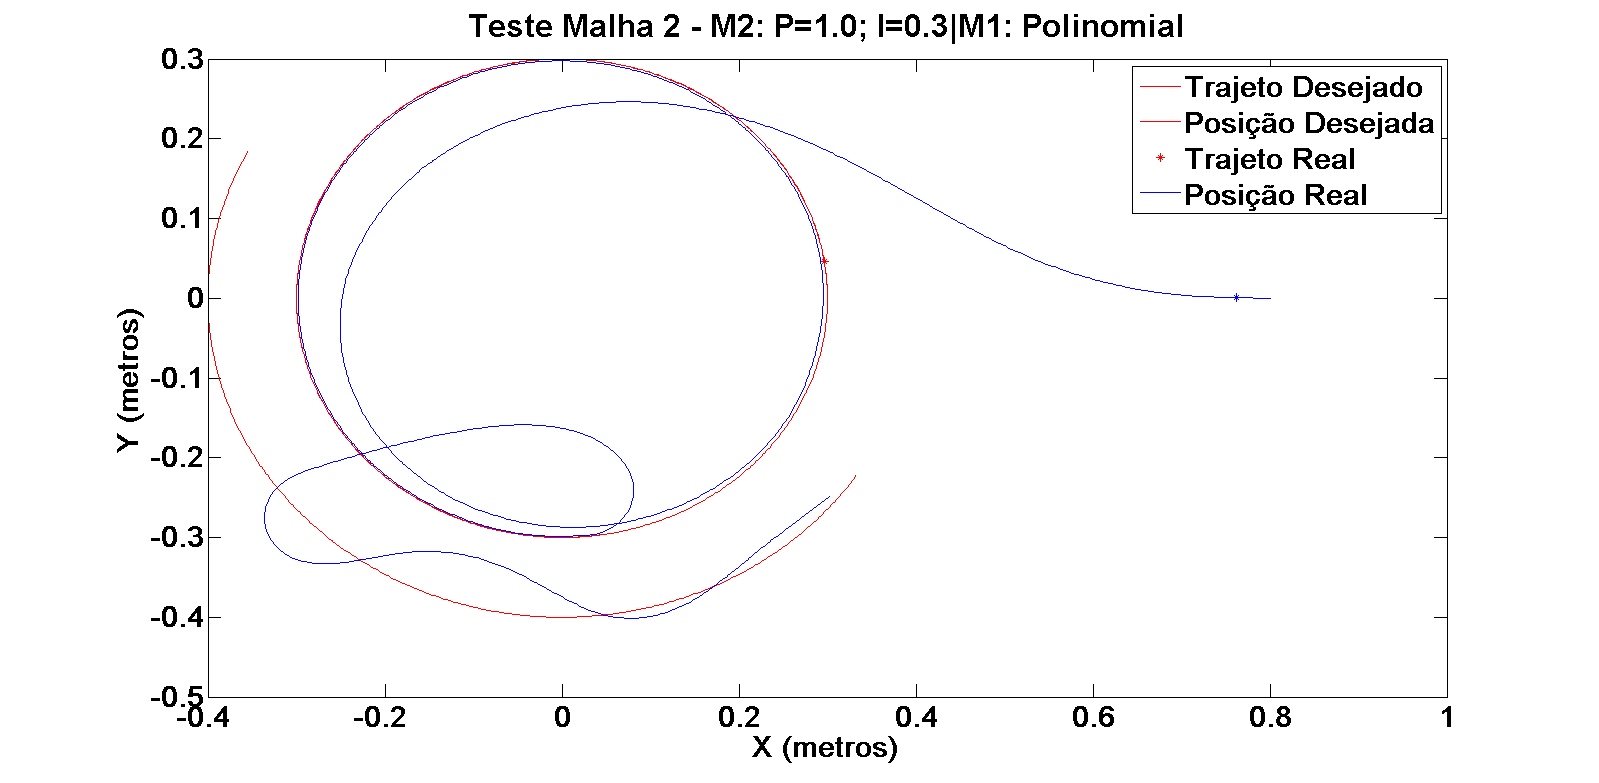
\includegraphics[width=.9\linewidth]{./Testes/Malha2/P1.0I0.3/IntegralOsc}
    		\caption{Malha Intermediária: P=1.0; I=0.3 - Malha Interna: Polinomial}
    		\label{fig:m2polpos2}
    	\end{subfigure}
    	\begin{subfigure}{1.0\textwidth}
    		\centering
    		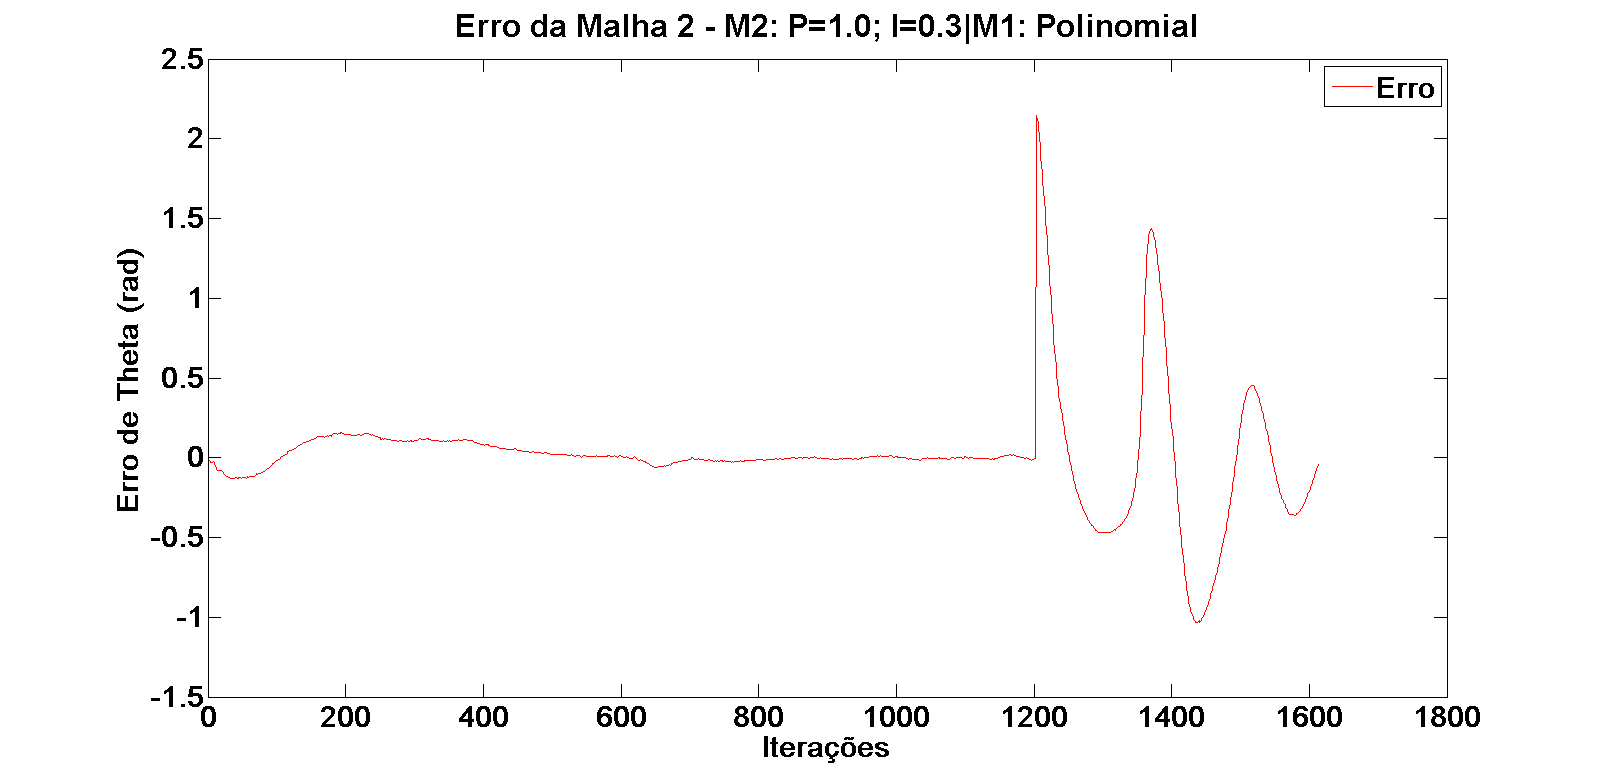
\includegraphics[width=.9\linewidth]{./Testes/Malha2/P1.0I0.3/ErroThetaIOsc}
    		\caption{Erro da Malha Intermediária: P=1.0; I=0.3 - Malha Interna: Polinomial}
    		\label{fig:m2piderr2}
    	\end{subfigure}
    	\caption{Experimentos com a Malha Intermediária com Controlador Proporcional e Malha Interna: Controlador Polinomial}
    	\label{fig:m2pol2}
    \end{figure}



